\scanpage{79}
\figure{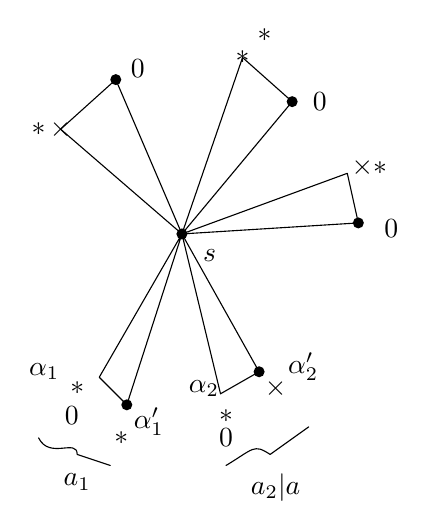
\begin{tikzpicture}[x=.07cm,y=-.07cm,line cap=round,line join=round]
\draw (36,36) -- (14,17) -- (24,8) -- cycle;
\draw (36,36) -- (47,4) -- (56,12) -- cycle;
\draw (36,36) -- (66,25) -- (68,34) -- cycle;
\draw (36,36) -- (50,61) -- (43,65) -- cycle;
\draw (36,36) -- (26,67) -- (21,62) -- cycle;
\node[inner sep=.5pt] at (10,17) {$*$};
\node[inner sep=.5pt] at (14,17) {$\times$};
\node[inner sep=.5pt] at (28,6) {$0$};
\node[inner sep=.5pt] at (47,4) {$*$};
\node[inner sep=.5pt] at (51,0) {$*$};
\node[inner sep=.5pt] at (61,12) {$0$};
\node[inner sep=.5pt] at (70,24) {$\times *$};
\node[inner sep=.5pt] at (74,35) {$0$};
\node[inner sep=.5pt] at (41,40) {$s$};
\node[inner sep=.5pt] at (11,61) {$\alpha_1$};
\node[inner sep=.5pt] at (17,64) {$*$};
\node[inner sep=.5pt] at (16,69) {$0$};
\node[inner sep=.5pt] at (30,70) {$\alpha'_1$};
\node[inner sep=.5pt] at (25,73) {$*$};
\node[inner sep=.5pt] at (53,64) {$\times$};
\node[inner sep=.5pt] at (58,60) {$\alpha'_2$};
\node[inner sep=.5pt] at (40,64) {$\alpha_2$};
\node[inner sep=.5pt] at (44,69) {$*$};
\node[inner sep=.5pt] at (44,73) {$0$};
\node[inner sep=.5pt] at (17,81) {$a_1$};
\node[inner sep=.5pt] at (53,82) {$\unsure{a_2|a}$};
\foreach \x/\y in {24/8,56/12,68/34,36/36,50/61,26/67}{\fill (\x,\y) circle (.07cm);}
\draw (10,73) .. controls (12,77) and (17,73) .. (17,76) -- (23,78);
\draw (44,78) .. controls (49,75) and (49,74) .. (52,76) -- (59,71);
\end{tikzpicture}}
\[
\begin{array}{l}M\subset\mathbb F_2^Q\\[-.3ex]\ \backslash\,P\end{array}
\]
\diagram{\begin{tikzcd}[ampersand replacement=\&,column sep=.5em,row sep=.5em]
\& {} \arrow[-]{r} \& {}\\
{} \arrow{ur} \arrow{r} \& {} \arrow{ur}\&
\end{tikzcd}}
$Q$ ens de card $5$

$I\unsure{\subset|\in} Q$ ens de cardinal $2$
\[
\begin{array}{l@{\qquad}l@{\qquad}l}
e_i\in M&e_1,e_2\quad e_1+e_2&\\
\unsure{P|R}&e'_1=e_2+e_3+e_4+e_5&e_i+\mathbb{1}\qquad e_j+\mathbb{1}\\
&e'_2=e_1+e_3+e_4+e_5&e_i-e_j+\unsure{\mathbb Z|2}\\
&e'_1+e'_2=e_1+e_2&
\end{array}
\]
\figure{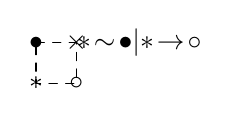
\begin{tikzpicture}[x=.032cm,y=-.032cm,line cap=round,line join=round]
\draw[dashed] (0,0) -- (16,0) -- (16,16) -- (0,16) -- cycle;
\node[inner sep=.5pt] at (0,0) {$\bullet$};
\node[inner sep=.5pt] at (16,0) {$\times$};
\node[inner sep=.5pt] at (0,16) {$*$};
\node[inner sep=.5pt] at (16,16) {$\circ$};
\node[inner sep=.5pt] at (41,0) {$\deleted{\unsure{*\!\sim\!\bullet|*\!\to\!\circ}}$};

\end{tikzpicture}}
\[
 e_i+\mathbb{1},\ e_j+\mathbb{1}\qquad e_i+e_j\qquad \mathbb F_2^I
\]
\diagram{\(\begin{array}{c|c|c|}&\alpha_1&\alpha'_1\\ \hline
\alpha_2&\circ&*\\ \hline
\alpha'_2&\times&\bullet\end{array}\)}
\diagram{\begin{tikzcd}[ampersand replacement=\&,row sep=.3em,column sep=1em]
\widetilde I^{\unsure{4|\ast}}\arrow{d}\&\\ I\&J\\ 2\&3
\end{tikzcd}}
\[
\begin{aligned}
&\deleted{\unsure{T|I}}\ \widetilde I\amalg(J\times\tau(\widetilde I/I))\\
&\underbrace{[0,1]}_{I_0}\amalg\underset{2}{I}_1\amalg(J\times I_1)
\end{aligned}
\]
\figure{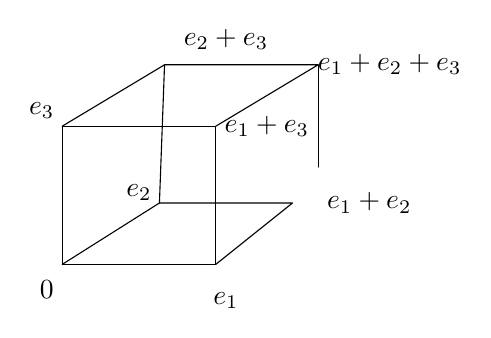
\begin{tikzpicture}[x=.065cm,y=-.065cm,line cap=round,line join=round]
\draw (0,21) -- (30,21) -- (30,48) -- (0,48) -- cycle;
\draw (0,21) -- (20,9) -- (50,9) -- (30,21);
\draw (0,48) -- (19,36) -- (45,36) -- (30,48);
\draw (19,36) -- (20,9);
\draw (50,9) -- (50,29);
\node[inner sep=.5pt] at (-3,53) {$0$};
\node[inner sep=.5pt] at (32,55) {$e_1$};
\node[inner sep=.5pt] at (15,34) {$e_2$};
\node[inner sep=.5pt] at (-4,18) {$e_3$};
\node[inner sep=.5pt] at (40,21) {$e_1+e_3$};
\node[inner sep=.5pt] at (60,36) {$e_1+e_2$};
\node[inner sep=.5pt] at (32,4) {$e_2+e_3$};
\node[inner sep=.5pt] at (64,9) {$e_1+e_2+e_3$};

\end{tikzpicture}}
\figure{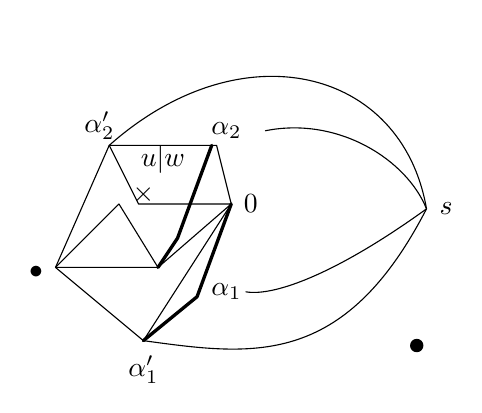
\begin{tikzpicture}[x=.062cm,y=-.062cm,line cap=round,line join=round]
\draw (4,37) -- (15,12) -- (37,12) -- (40,24) -- (22,52) -- cycle;
\draw (4,37) -- (25,37) -- (40,24);
\draw (15,12) -- (21,24) -- (40,24);
\draw (4,37) -- (17,24) -- (25,37);
\draw[very thick] (22,52) -- (33,43) -- (40,24);
\draw[very thick] (25,37) -- (29,31) -- (36,12);
\node[inner sep=.5pt] at (0,38) {$\bullet$};
\node[inner sep=.5pt] at (13,8) {$\alpha'_2$};
\node[inner sep=.5pt] at (39,9) {$\alpha_2$};
\node[inner sep=.5pt] at (44,24) {$0$};
\node[inner sep=.5pt] at (39,42) {$\alpha_1$};
\node[inner sep=.5pt] at (22,58) {$\alpha'_1$};
\node[inner sep=.5pt] at (84,25) {$s$};
\node[inner sep=.5pt] at (22,22) {$\times$};
\node[inner sep=.5pt] at (26,15) {$\unsure{u|w}$};
\draw (15,12) .. controls (42,-12) and (75,-4) .. (80,25) .. controls (63,58) and (44,55) .. (22,52);
\draw (47,9) .. controls (62,6) and (76,15) .. (80,25) .. controls (62,38) and (49,43) .. (43,42);
\fill (78,53) circle (.085cm);
\end{tikzpicture}}
\figure{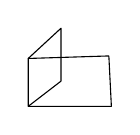
\begin{tikzpicture}[x=.032cm,y=-.032cm,line cap=round,line join=round]
\draw (0,12) -- (32,11) -- (33,31) -- (0,31) -- cycle;
\draw (0,12) -- (13,0) -- (13,21) -- (0,31);


\end{tikzpicture}}
\figure{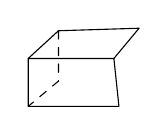
\begin{tikzpicture}[x=.032cm,y=-.032cm,line cap=round,line join=round]
\draw (0,12) -- (34,12) -- (36,31) -- (0,31) -- cycle;
\draw (0,12) -- (12,1) -- (44,0) -- (34,12);
\draw[dashed] (12,1) -- (12,21) -- (0,31);


\end{tikzpicture}}
\[
 e_1,\ e_2,\ e_3\qquad\deleted{\unsure{I\amalg I|2+2}}\ \mathbb F_2^J
\]
\figure{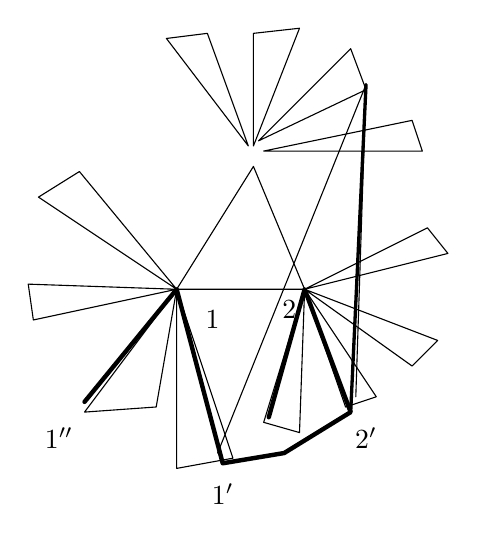
\begin{tikzpicture}[x=.065cm,y=-.065cm,line cap=round,line join=round]
\draw (30,56) -- (45,32) -- (55,56) -- cycle;
\draw (30,56) -- (3,38) -- (11,33) -- cycle;
\draw (30,56) -- (1,55) -- (2,62) -- cycle;
\draw (30,56) -- (12,80) -- (26,79) -- cycle;
\draw (30,56) -- (30,91) -- (41,89) -- cycle;
\draw (55,56) -- (79,44) -- (83,49) -- cycle;
\draw (55,56) -- (81,66) -- (76,71) -- cycle;
\draw (55,56) -- (69,77) -- (63,79) -- cycle;
\draw (55,56) -- (54,84) -- (47,82) -- cycle;
\draw (44,28) -- (28,7) -- (36,6) -- cycle;
\draw (45,28) -- (45,6) -- (54,5) -- cycle;
\draw (46,27) -- (64,9) -- (67,17) -- cycle;
\draw (47,29) -- (76,23) -- (78,29) -- cycle;
\draw (38,88) -- (67,16) -- (65,77);
\draw[ultra thick] (12,78) -- (30,56) -- (39,90) -- (51,88) -- (64,80) -- (55,56) -- (48,81);
\draw[very thick] (64,80) -- (67,16);
\node[inner sep=.5pt] at (37,62) {$1$};
\node[inner sep=.5pt] at (52,60) {$2$};
\node[inner sep=.5pt] at (7,85) {$1''$};
\node[inner sep=.5pt] at (39,96) {$1'$};
\node[inner sep=.5pt] at (67,85) {$2'$};

\end{tikzpicture}}
\[
\begin{aligned}
&3.2^6\qquad3.2^3\qquad3.2=6.\quad 2\\
&1''\quad\inserted{\text{lié : }1}\quad\text{non lié : }2'\ (\text{ou : }1')\\
&2''\ \deleted{\unsure{\sim|u}}\left\{\begin{array}{ll}\text{lié :}&2\\
\text{lié :}&1''.\\ \text{non lié :}&1',2'\end{array}\right.\\
&\left\{\begin{array}{l}\deleted{\text{lié}}\quad\deleted{\unsure{6|G|\in}}\unsure{\overline E(2)^*|E(2)^+|\widehat E(2)^*}\\
\text{lié : }1''\text{ et }\sigma1',\\
\ne\sigma2'\end{array}\right.
\end{aligned}
\]
\diagram{\begin{tikzcd}[ampersand replacement=\&,row sep=.6em,column sep=.9em]
\& w\&\sigma_4\&\\
\&u\arrow[-]{r}\arrow[-]{dl}\arrow[-]{d}\&v\arrow[-]{d}\arrow[-]{dr}\&\\
\alpha'_3\&\alpha_4\arrow[-]{r}\&\beta_4\&{}
\end{tikzcd}}
\diagram{\begin{tikzcd}[ampersand replacement=\&,row sep=.8em,column sep=.8em]
\&u\arrow[-]{r}\arrow[-]{dl}\arrow[-]{d}\&v\arrow[-]{dl}\arrow[-]{dr}\&\\
\alpha'_3\arrow[-]{r}\&\beta_3\arrow[-]{r}\&\alpha_4\arrow[-]{r}\&\beta_4
\end{tikzcd}}
\diagram{\begin{tikzcd}[ampersand replacement=\&,row sep=.6em,column sep=.5em]
\&\&\gamma_4\arrow[-]{d}\arrow[-]{dddll}\arrow[-,bend left=30]{ddd}\&\\
\&\&w\arrow[-]{dl}\arrow[-]{dr}\&\\
\&u\arrow[-]{rr}\arrow[-]{dl}\arrow[-]{d}\&\&v\arrow[-]{dl}\arrow[-]{d}\\
\alpha'_3\&\alpha_4\&\beta_3\&\beta_4
\end{tikzcd}}
\figure{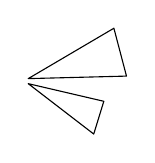
\begin{tikzpicture}[x=.032cm,y=-.032cm,line cap=round,line join=round]
\draw (0,20) -- (34,0) -- (39,19) -- cycle;
\draw (0,22) -- (30,29) -- (26,42) -- cycle;


\end{tikzpicture}}
\figure{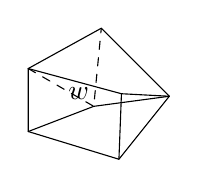
\begin{tikzpicture}[x=.032cm,y=-.032cm,line cap=round,line join=round]
\draw (0,16) -- (29,0) -- (56,27) -- (36,52) -- (0,41) -- cycle;
\draw (0,16) -- (37,26) -- (56,27);
\draw (37,26) -- (36,52);
\draw (0,41) -- (26,31) -- (56,27);
\draw[dashed] (0,16) -- (26,31) -- (29,0);
\node[inner sep=.5pt] at (20,26) {$w$};

\end{tikzpicture}}
\[
\begin{array}{c@{\qquad}cccc}
 \alpha'_3&\beta'_1&\beta'_2&\beta^{\unsure{\ast|1|\prime}}_3&\beta'_4\\
 \alpha'_4&\beta^{\unsure{\ast|1}}_1&\beta_2&\beta^1_3&\beta'_4
\end{array}\qquad 2.6.8
\]
% archive sheet number: 78
